\documentclass[9pt,twocolumn,twoside,]{pnas-new}

% Use the lineno option to display guide line numbers if required.
% Note that the use of elements such as single-column equations
% may affect the guide line number alignment.


\usepackage[T1]{fontenc}
\usepackage[utf8]{inputenc}

% tightlist command for lists without linebreak
\providecommand{\tightlist}{%
  \setlength{\itemsep}{0pt}\setlength{\parskip}{0pt}}


% Pandoc citation processing
%From Pandoc 3.1.8
% definitions for citeproc citations
\NewDocumentCommand\citeproctext{}{}
\NewDocumentCommand\citeproc{mm}{%
  \begingroup\def\citeproctext{#2}\cite{#1}\endgroup}
\makeatletter
 % allow citations to break across lines
 \let\@cite@ofmt\@firstofone
 % avoid brackets around text for \cite:
 \def\@biblabel#1{}
 \def\@cite#1#2{{#1\if@tempswa , #2\fi}}
\makeatother
\newlength{\cslhangindent}
\setlength{\cslhangindent}{1.5em}
\newlength{\csllabelwidth}
\setlength{\csllabelwidth}{3em}
\newenvironment{CSLReferences}[2] % #1 hanging-indent, #2 entry-spacing
 {\begin{list}{}{%
  \setlength{\itemindent}{0pt}
  \setlength{\leftmargin}{0pt}
  \setlength{\parsep}{0pt}
  % turn on hanging indent if param 1 is 1
  \ifodd #1
   \setlength{\leftmargin}{\cslhangindent}
   \setlength{\itemindent}{-1\cslhangindent}
  \fi
  % set entry spacing
  \setlength{\itemsep}{#2\baselineskip}}}
 {\end{list}}
\usepackage{calc}
\newcommand{\CSLBlock}[1]{#1\hfill\break}
\newcommand{\CSLLeftMargin}[1]{\parbox[t]{\csllabelwidth}{#1}}
\newcommand{\CSLRightInline}[1]{\parbox[t]{\linewidth - \csllabelwidth}{#1}\break}
\newcommand{\CSLIndent}[1]{\hspace{\cslhangindent}#1}


\templatetype{pnasresearcharticle}  % Choose template

\title{Variations spatio-temporelles de la biodiversité des lépidoptères
au Québec}

\author[a]{Marika Roberge}
\author[a]{Bertrand Labrecque}
\author[a]{Juliette Boulet-Thomas}

  \affil[a]{Faculté des sciences, Département de biologie, 2500
Boulevard de l'Université, Sherbrooke, Québec, J1K 2R1}


% Please give the surname of the lead author for the running footer
\leadauthor{Roberge}

% Please add here a significance statement to explain the relevance of your work
\significancestatement{}


\authorcontributions{}



\correspondingauthor{\textsuperscript{} }

% Keywords are not mandatory, but authors are strongly encouraged to provide them. If provided, please include two to five keywords, separated by the pipe symbol, e.g:
 \keywords{  lepidopteres |  communautés |  variation
temporelle |  variation spatiale  } 

\begin{abstract}
Inclure le résumé ici.
\end{abstract}

\dates{This manuscript was compiled on \today}
\doi{\url{www.pnas.org/cgi/doi/10.1073/pnas.XXXXXXXXXX}}

\begin{document}

% Optional adjustment to line up main text (after abstract) of first page with line numbers, when using both lineno and twocolumn options.
% You should only change this length when you've finalised the article contents.
\verticaladjustment{-2pt}



\maketitle
\thispagestyle{firststyle}
\ifthenelse{\boolean{shortarticle}}{\ifthenelse{\boolean{singlecolumn}}{\abscontentformatted}{\abscontent}}{}

% If your first paragraph (i.e. with the \dropcap) contains a list environment (quote, quotation, theorem, definition, enumerate, itemize...), the line after the list may have some extra indentation. If this is the case, add \parshape=0 to the end of the list environment.

\acknow{}

\section{Introduction et questions de
recherche}\label{introduction-et-questions-de-recherche}

Les lépidoptères, en tant qu'indicateurs sensibles à la température et
aux changements environnementaux (1, 2), sont particulièrement utiles
pour évaluer les effets des perturbations anthropiques, notamment les
changements climatiques et l'altération des habitats. Au Québec,
plusieurs espèces pourraient voir leur aire de répartition modifiée,
soit par l'expansion d'espèces thermophiles vers le nord, soit par un
recul des espèces froid-adaptées.

Dans ce contexte, nous avons étudié l'évolution de la diversité des
lépidoptères au Québec, à la fois dans le temps et dans l'espace, en
nous basant sur les données de présence collectées depuis environ 150
ans. L'objectif principal est d'évaluer les changements dans la
diversité des lépidoptères au Québec à travers ces deux dimensions.
Ainsi, la première analyse se pose la question suivante : comment la
richesse spécifique des lépidoptères a-t-elle évolué au fil des années ?
La deuxième analyse s'interroge sur : comment la diversité et la
répartition des lépidoptères ont-elles évolué au fil du temps et selon
les régions du Québec ? Enfin, la troisième analyse cherche à répondre à
la question suivante : comment la répartition de Papilio canadensis
a-t-elle changé au cours du temps et dans l'espace au Québec ?

Ces résultats permettront de discuter des mécanismes potentiels à
l'origine des patrons observés, entre biais d'échantillonnage et signaux
biologiques réels, et d'évaluer si la composition des communautés de
lépidoptères au Québec reflète une transformation de la biodiversité
entomologique.

\section{Méthode et résultats
d'analyse}\label{muxe9thode-et-ruxe9sultats-danalyse}

Ici, est présenté un graphique (Fig. 1) mettant en évidence les
variations en termes de nombre d'espèces uniques observés au fil des
années. Expliquer pourquoi le nombre unique est utiliser et donc sa
pertinence.

\begin{figure}
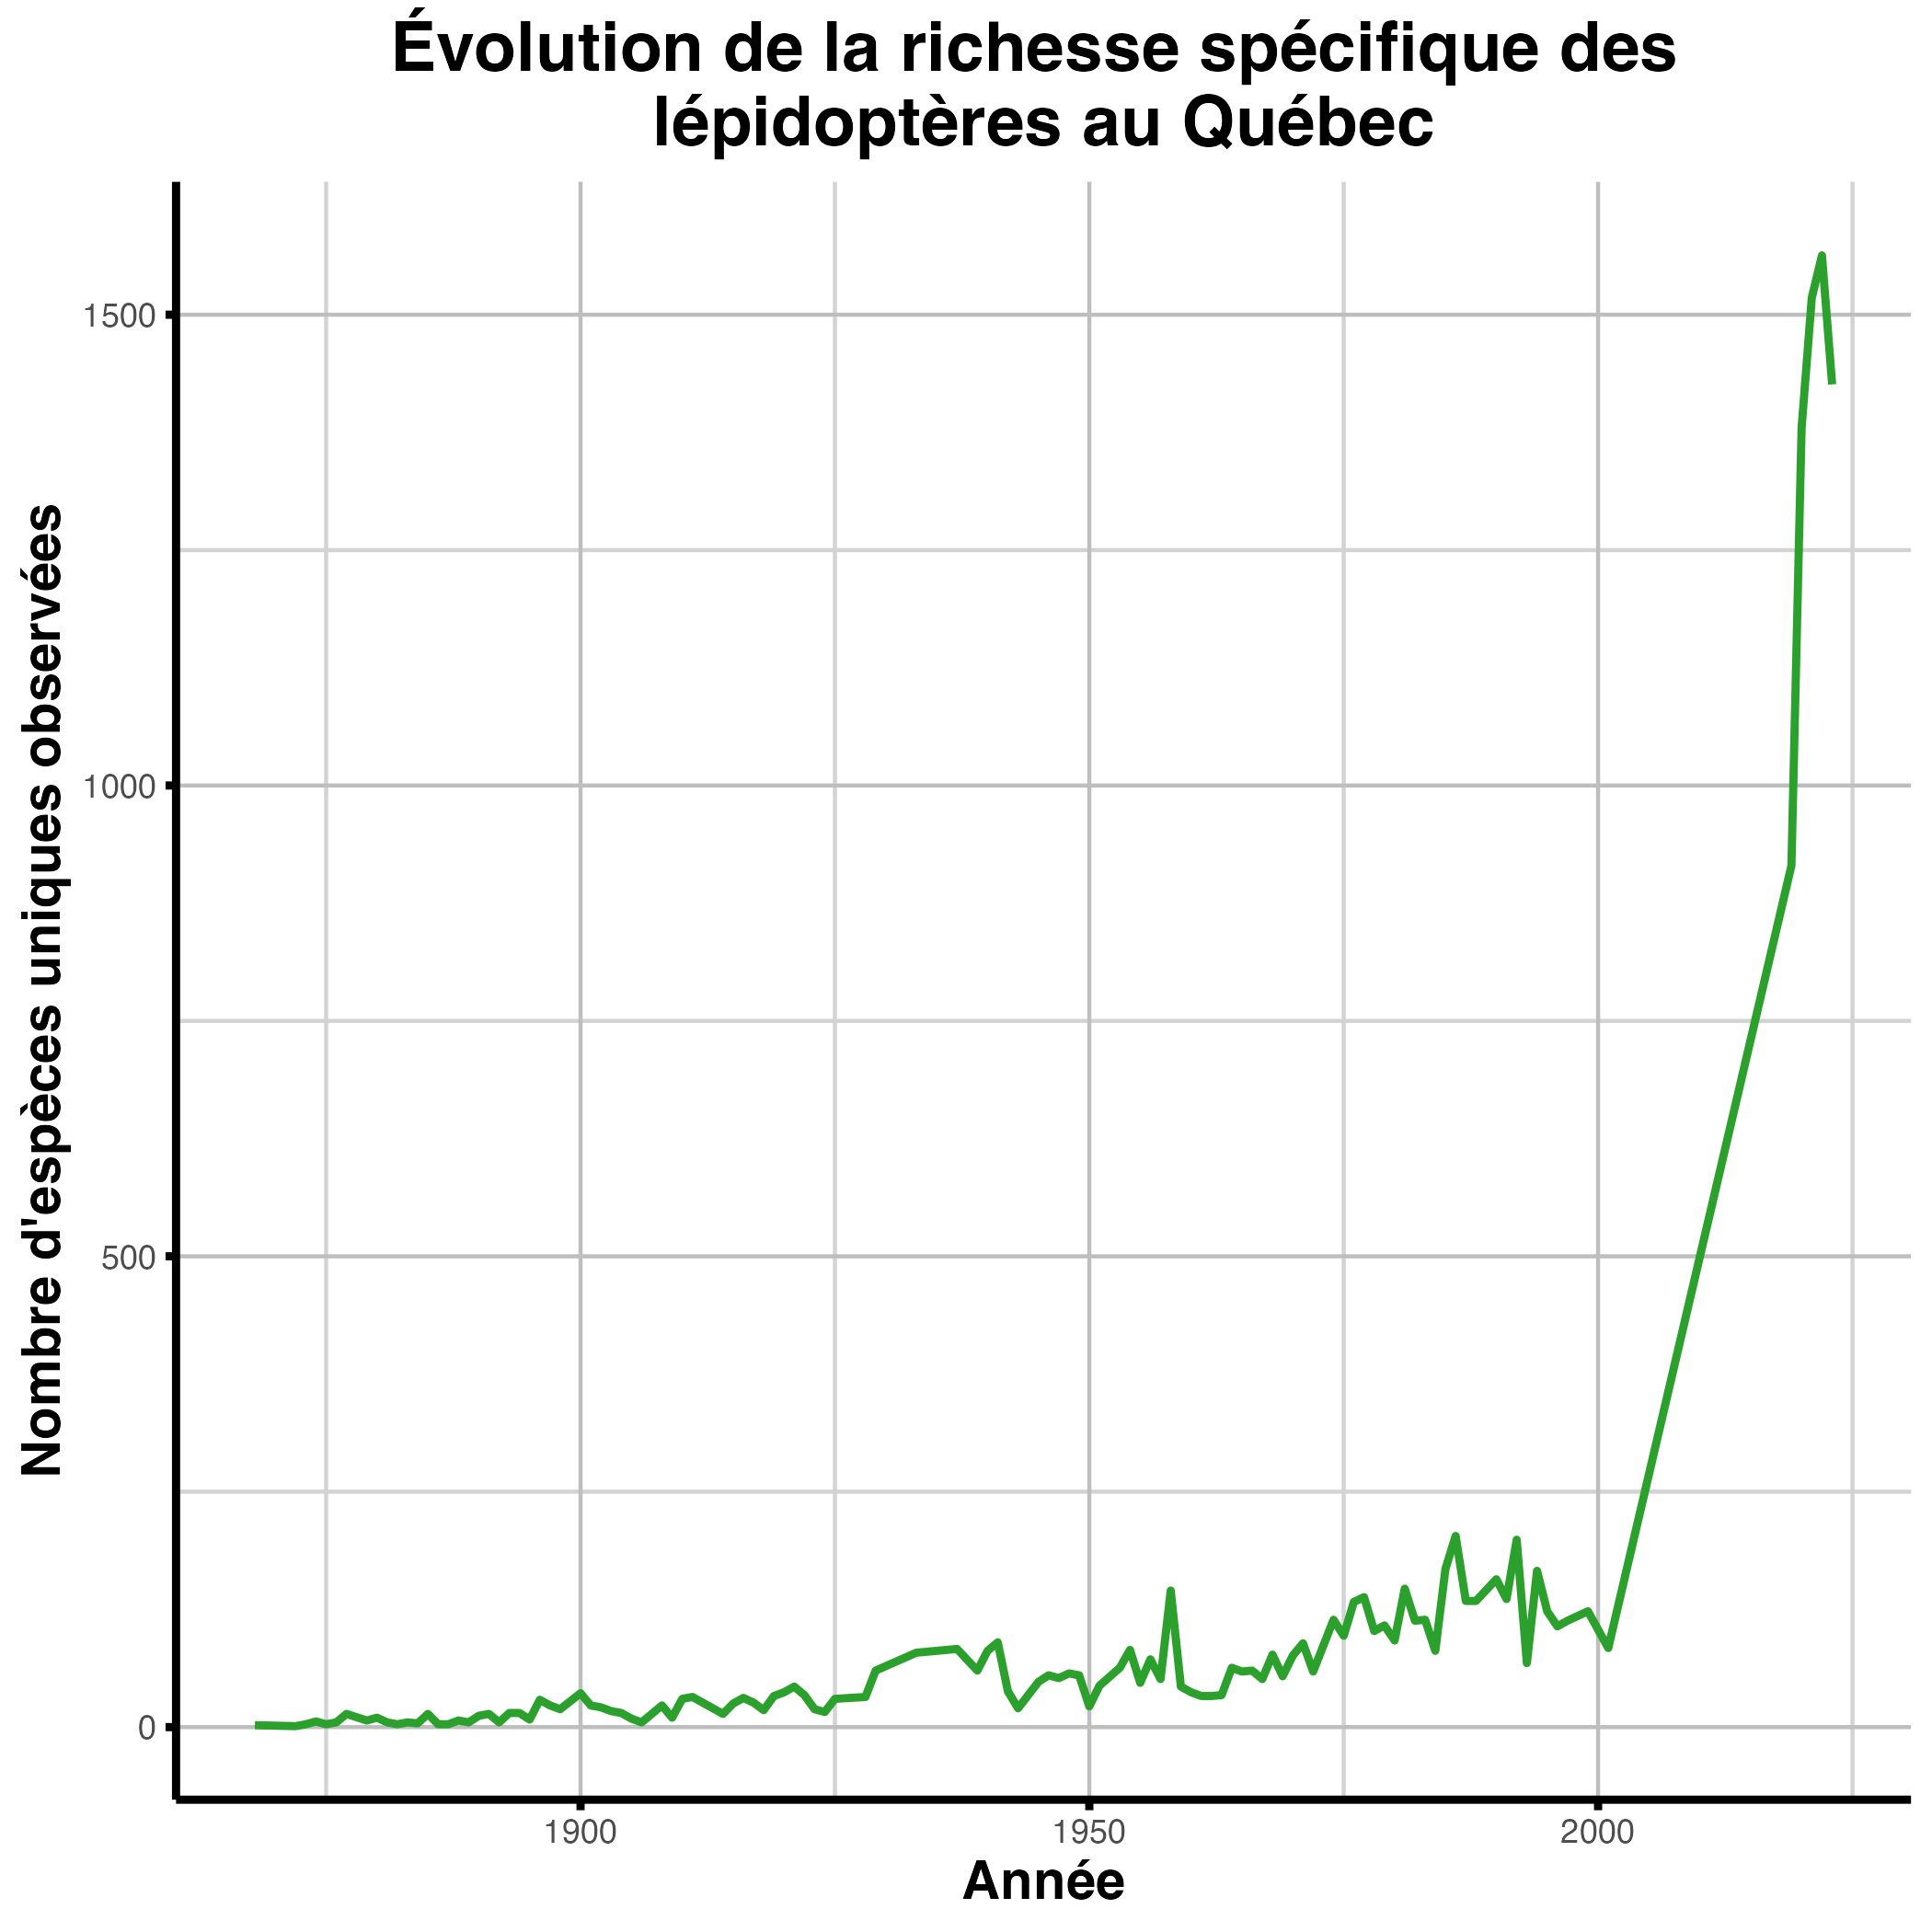
\includegraphics[width=0.9\linewidth]{../Figures_analyse/graphique_biodiversite} \caption{Variation du nombre d'espèces de lépidoptères au Québec en fonction du temps.}\label{fig:fig_graphique_biodiversite}
\end{figure}

Comme deuxième analyse, elle porte sur une espèce commune au Québec,
Papilio canadensis, communément appelé Papillon tigré du Canada (Fig.
2). Présenter ici la biologie de l'espèce rapidement et de combien de
données ont a utilisés pour créer le graphique. Avec références
bibliographiques.

\begin{figure}
\centering
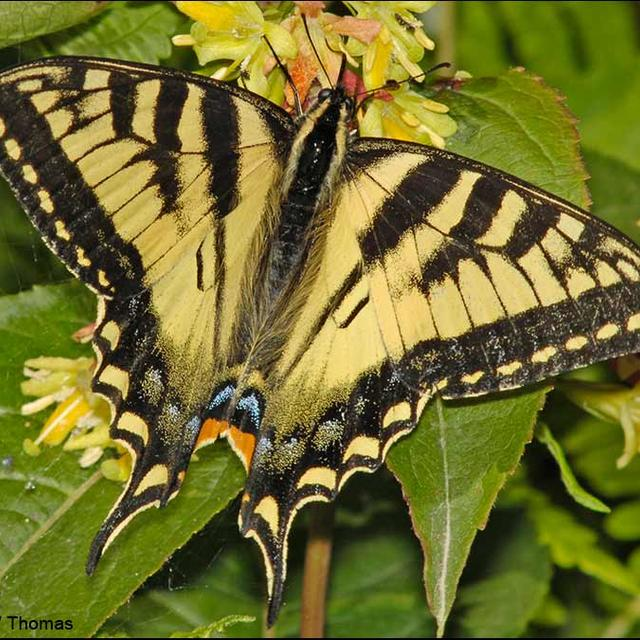
\includegraphics{Papilio_canadensis.png}
\caption{Papillon tigré du Canada (\emph{Papilio canadensis}) observé
dans son habitat naturel.}
\end{figure}

L'analyse portant sur l'espèce permet de décrire comment la répartition
de \emph{Papilio canadensis} change dans le temps et l'espace.

!{[}Répartition de Papilio canadensis au Québec au fil des années.span
data-label=figpapiliospan{]} \#ajouter un png de notre figure obtenue
dans un code chunk comme les autres figures d'analyse.

Texte ici présentant les résultats de l'analyse 2.Comme on peut le voir
sur la Figure 2, on voit que la répartition de \emph{P. canadensis}
s'est\ldots{}

On voit dans cette figure (Fig.3 - ici cartes de l'espece) que \ldots On
peut donc dire que l'espèce est devenue plusmoins présente avec le
temps\ldots{}

Maintenant, dans cette section, nous analysons l'évolution de la
biodiversité des lépidoptères au fil du temps à travers plusieurs
visualisations. Nous allons créer des cartes et des graphiques pour
observer les variations et tendances.

Pour l'étude de la biodiversité des lépidoptères dans le temps et
l'espace, une figure regroupant six cartes a été réalisée. Dans cette
figure, on observe la carte de la province du Québec qui est notre aire
d'étude principale. Les points géographiques de la base de données qui
sont à l'extérieur de la province ne sont pas pris en compte. La carte
la plus ancienne débute en 1875 et représente les données sur 25 ans,
soit de 1875 jusqu'à la fin de 1879, ces bonds de 25 ans de données vont
jusqu'aux données les plus récentes, soit en 2024. Cette image permet
donc de combiner une analyse temporelle (par tranche de 25 ans) et une
agrégation spatiale via une grille hexagonale. En effet, une grille
hexagonable est utilisée pour éviter les effets de bord qu'on a avec une
grille carrée. De plus, elle permet une meilleure agrégration spatiale.
La projection utilisée pour cette carte est EPSG 32198, qui est la
projection locale du Québec. Cela permet une représentation précise à
l'échelle régionale. Pour finir, une moyenne de nombre d'espèces par
cellule pour chaque période de temps a été fait. Ce qui donne une idée
plus stable et comparable de la diversité à travers le temps. En
conclusion, ces 6 cartes sont combinées en une seule image finale, ce
qui permet une comparaison visuelle claire de l'évolution
spatio-temporelle de la diversité spécifique au Québec. Ce qui est utile
visualiser les zones où la diversité augmente, diminue ou reste stable.

La Figure 4 ci-dessous montrent l'évolution de la biodiversité des
lépidoptères pour différentes périodes et critères.

\begin{figure}

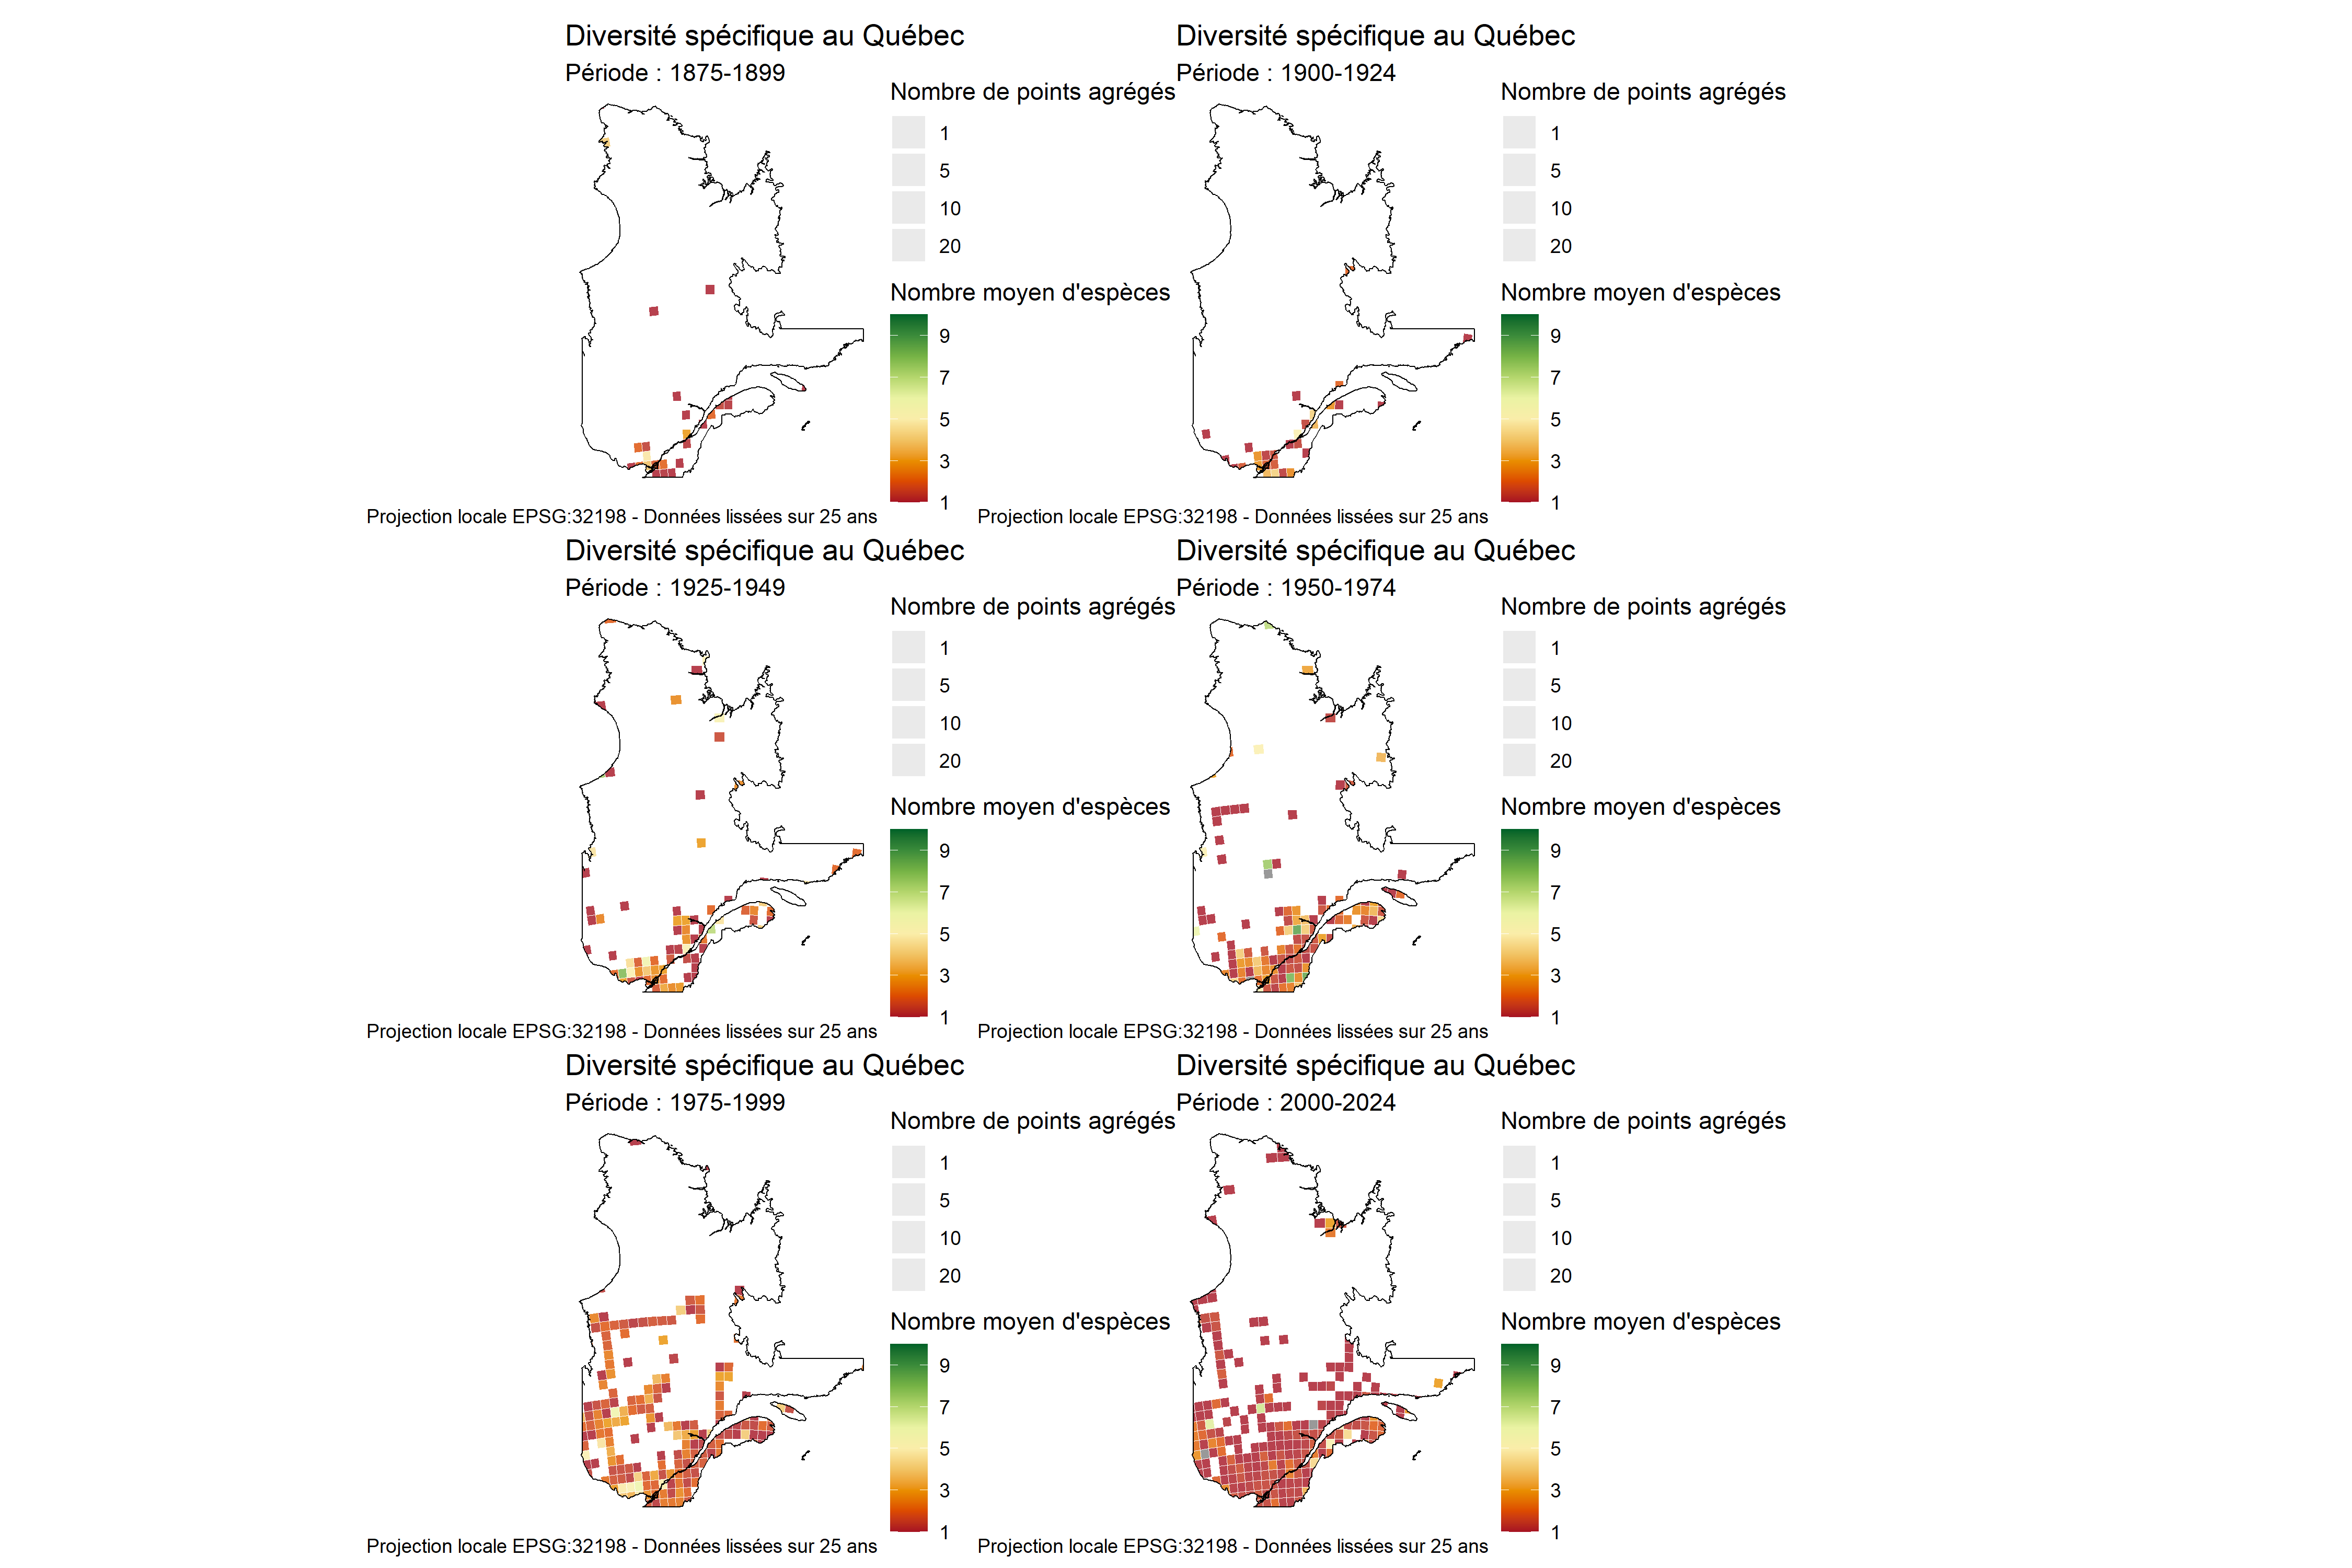
\includegraphics[width=1\linewidth]{../Figures_analyse/cartes_combinees} \hfill{}

\caption{Image de la province du Québec et de six cartes qui montrent l'évolution de la biodiversité des espèces de lépidoptères au fil du temps (fenêtres de 25 ans).}\label{fig:fig_cartes_combinees, fullpage-figure}
\end{figure}

Ces cartes montrent une augmentation de la couverture spatio-temporelle
des données au fil des décennies. Plus on avance dans le temps, plus il
y a des cellules remplies et plus les données sont denses et complètes.
On voit aussi une légère augmentation du nombre d'espèces dans certaines
régions, mais cette tendance est influencée par autre chose.

Un premier point important a aborder est que entre 1975 et 1899 il y a
très peu de données et celle-ci sont concetrées autour de grandes villes
comme Montréal, Québec, Sherbrooke, etc. La diversité moyenne pour cette
période est faible à modérée, mais les données sont trop rares pour
conclure quelques choses. Si on s'attarde entre 1900-1934 et 1925-1949,
on remarque une progression lente de la couverture via les données
d'échantillonnage. Il y a encore peu d'échantillons, donc les valeurs de
diveristé sont peu fiables. Les zones urbaines du sud par contre sont
bien couvertes. De 1950-1974, on voit une nette amélioration de la
couverture, des cellules commencent à atteindre une diversité de 7-9
espèces en moyenne dans le sud de la province. Par contre, de 1975-1999,
il y a un essort de données. La majorité du sud du Québec est maintenant
couverte, surtout autour des grands centres et zones garicoles. On
remarque aussi plus de verts ce qui indique une augmentation du nombre
d'espèces osbervées. Pour notre dernière plage de temps, de 2000-2024,
il y a une couverture plus dense et étendue. La diversité moyenne est
plus élevée dans plusieurs régions. Cela est probablement lié à une
explosion des efforts de suivi, l'arrivée de bases de données en ligne
comme iNaturalist.

\section{Discussion}\label{discussion}

-Analyse 1 : -Analyse 2 : -Analyse 3 : Un biais de la cartes de
biodiversité spatio-temporelle est que plus on avance dans le temps plus
il y a d'observation ce qui est logique. Par contre, ces données
reflètent aussi les efforts d'échantillonnage autant que la réalité
biologique. Ce qui mène aussi à se poser la question pour les zones en
rouges (faible diversité), à savoir si elles représentent réellement peu
d'espèces ou simplement un manque de points d'échantillonnage. De plus,
le sud du Québec a plus de données récoltées et c'est aussi là qu'on
remarque une augmentation de la diversité. D'autre part, à partir de
1975, on voit une bonne stabilisation du nombre d'espèces moyen dans
plusieurs cellules, ce qui pourrait refléter un effort d'échantillonnage
suffisant pour capter la vraie diversité locale.

\section{Conclusion}\label{conclusion}

\showmatmethods
\showacknow
\pnasbreak

\phantomsection\label{refs}
\begin{CSLReferences}{0}{1}
\bibitem[\citeproctext]{ref-devictor_differences_2012}
\CSLLeftMargin{1. }%
\CSLRightInline{Devictor V, et al. (2012)
\href{https://doi.org/10.1038/NCLIMATE1347}{Differences in the climatic
debts of birds and butterflies at a continental scale}. \emph{Nature
Climate Change} 2:121--124.}

\bibitem[\citeproctext]{ref-parmesan_poleward_1999}
\CSLLeftMargin{2. }%
\CSLRightInline{Parmesan C, et al. (1999)
\href{https://doi.org/10.1038/21181}{Poleward shifts in geographical
ranges of butterfly species associated with regional warming}.
\emph{Nature} 399(6736):579--583.}

\end{CSLReferences}



% Bibliography
% \bibliography{pnas-sample}

\end{document}
